\documentclass{article}

\usepackage{a4}
\usepackage{amsmath}
\usepackage{amssymb}
\usepackage{ctex}
\usepackage{booktabs}
\usepackage{graphicx}
\usepackage{subfigure}
\usepackage{subcaption}
\usepackage{float}
\usepackage{hyperref}
\usepackage{xurl}
\usepackage{enumitem}
\usepackage{array}
\usepackage{longtable}
\usepackage{multirow}
\usepackage{fvextra}

\hypersetup{colorlinks=true,linkcolor=black,urlcolor=blue,citecolor=black}
\setlist[itemize]{nosep,leftmargin=1.8em}
\setlist[enumerate]{nosep,leftmargin=1.8em}
\captionsetup{font=small}
\RecustomVerbatimEnvironment{verbatim}{Verbatim}{
  breaklines=true,
  breakanywhere=true,
  fontsize=\small
}

\title{计算机组成原理 \\ 实验5 单周期CPU指令扩展}
\author{鲁昕宁 2414015}
\date{\today}

\begin{document}

\maketitle
\begin{center}
    \url{https://github.com/SidneyLu/Computer-Organization-and-Design-NKU-CS/tree/master/lab6}
\end{center}

\newpage

\section{实验目标}
参考实验指导手册第六次单周期CPU实验，完成以下改进：
\begin{enumerate}
    \item 在现有CPU上新增两条指令：\texttt{sub}（R型）与\texttt{bgtz}（I型）；
    \item 用MIPS汇编编写一个计算斐波那契数列的程序，在\texttt{inst\_rom.v}中按照附件逻辑实现\texttt{Fib(10)}计算；
    \item 满足“\texttt{00H~48H}原有指令不改、原\texttt{4CH: j 00H}放到新增段末尾”的要求。
\end{enumerate}

\section{实验原理}

\subsection{新增指令语义}
\begin{enumerate}
    \item \textbf{sub rd, rs, rt}：\texttt{GPR[rd] = GPR[rs] - GPR[rt]}。
    \item \textbf{bgtz rs, offset}：当\texttt{GPR[rs] > 0}时分支到目标地址。
\end{enumerate}

\subsection{控制通路改动}
\begin{enumerate}
    \item 在译码中增加\texttt{inst\_SUB}和\texttt{inst\_BGTZ}识别信号；
    \item 在分支判断中增加\texttt{bgtz\_taken=(~rs\_value[31]) \& (|rs\_value)}；
    \item 在写回集合中将\texttt{sub}并入R型写回；
    \item 为容纳\texttt{4CH}后的扩展代码，将指令ROM地址由\texttt{[6:2]}扩展为\texttt{[7:2]}（即索引位宽5->6）。
\end{enumerate}

\subsection{Fib(10)汇编实现}
\begin{verbatim}
Init:
  GPR[13] = 10   // n
  GPR[14] = 3    // idx
  GPR[15] = 1    // fib(1)
  GPR[16] = 1    // fib(2)
  GPR[17] = GPR[15] + GPR[16]

Loop:
  GPR[14] = GPR[14] + 1
  GPR[15] = GPR[16]
  GPR[16] = GPR[17]
  GPR[17] = GPR[15] + GPR[16]
  GPR[18] = GPR[13] - GPR[14]
  if (GPR[18] > 0) goto Loop

  Mem[1] = GPR[17]
\end{verbatim}

\begin{verbatim}
# 依据实验附件示意图：使用 sub 与 bgtz 计算 Fib(10)
# 寄存器约定：
#   $13 = n(10)
#   $14 = idx(3)
#   $15 = fib(1)
#   $16 = fib(2)
#   $17 = 当前fib值
#   $18 = n - idx

.text
.globl main
main:
    # Init
    addiu $13, $0, 10      # GPR[13] = n = 10
    addiu $14, $0, 3       # GPR[14] = idx = 3
    addiu $15, $0, 1       # GPR[15] = fib(1) = 1
    addiu $16, $0, 1       # GPR[16] = fib(2) = 1
    addu  $17, $15, $16    # GPR[17] = fib(3)

loop:
    addiu $14, $14, 1      # GPR[14] = GPR[14] + 1
    addu  $15, $16, $0     # GPR[15] = GPR[16]
    addu  $16, $17, $0     # GPR[16] = GPR[17]
    addu  $17, $15, $16    # GPR[17] = GPR[15] + GPR[16]
    sub   $18, $13, $14    # GPR[18] = GPR[13] - GPR[14]
    bgtz  $18, loop        # 若 GPR[18] > 0 则跳转 loop

    sw    $17, 4($0)       # Mem[1] = GPR[17] = Fib(10)

halt:
    j halt
\end{verbatim}

\section{实验过程}

\subsection{源码修改}
\subsubsection{single\_cycle\_cpu.v}
\begin{verbatim}
assign inst_SUB   = op_zero & sa_zero    & (funct == 6'b100010);
assign inst_BGTZ  = (op == 6'b000111) & (rt == 5'd0);

assign bgtz_taken = (~rs_value[31]) & (|rs_value);

assign jbr_taken = j_taken
                 | (inst_BEQ  & beq_taken)
                 | (inst_BNE  & bne_taken)
                 | (inst_BGTZ & bgtz_taken);

assign inst_sub = inst_SUBU | inst_SUB;
assign inst_wdest_rd = inst_ADDU | inst_SUBU | inst_SUB | ... ;

// ROM地址扩展
.addr (inst_addr[7:2])
\end{verbatim}

\subsubsection{inst\_rom.v（关键地址）}
\begin{verbatim}
// 00H~48H 保持原样
inst_rom[18] = 32'h3C0C000C; // 48H: lui $12,#12

// 原4CH跳到新增Fib段
inst_rom[19] = 32'h08000014; // 4CH: j 50H

// 50H~80H 新增Fib代码
inst_rom[20] = 32'h240D000A; // addiu $13,$0,#10
inst_rom[21] = 32'h240E0003; // addiu $14,$0,#3
inst_rom[22] = 32'h240F0001; // addiu $15,$0,#1
inst_rom[23] = 32'h24100001; // addiu $16,$0,#1
inst_rom[24] = 32'h01F08821; // addu  $17,$15,$16
inst_rom[25] = 32'h25CE0001; // addiu $14,$14,#1
inst_rom[26] = 32'h02007821; // addu  $15,$16,$0
inst_rom[27] = 32'h02208021; // addu  $16,$17,$0
inst_rom[28] = 32'h01F08821; // addu  $17,$15,$16
inst_rom[29] = 32'h01AE9022; // sub   $18,$13,$14
inst_rom[30] = 32'h1E40FFFA; // bgtz  $18,64H
inst_rom[31] = 32'hAC110004; // sw    $17,#4($0)

// 把原4CH的 j 00H 放到新增段末尾
inst_rom[32] = 32'h08000000; // j 00H
\end{verbatim}

\subsection{仿真源码与结果}
\begin{verbatim}
`timescale 1ns / 1ps

module tb;

    reg clk;
    reg resetn;
    reg [4:0] rf_addr;
    reg [31:0] mem_addr;
    integer i;

    wire [31:0] rf_data;
    wire [31:0] mem_data;
    wire [31:0] cpu_pc;
    wire [31:0] cpu_inst;

    localparam [31:0] FIB10_EXPECT = 32'd55;

    single_cycle_cpu uut (
        .clk(clk),
        .resetn(resetn),
        .rf_addr(rf_addr),
        .mem_addr(mem_addr),
        .rf_data(rf_data),
        .mem_data(mem_data),
        .cpu_pc(cpu_pc),
        .cpu_inst(cpu_inst)
    );

    initial begin
        clk = 1'b0;
        resetn = 1'b0;
        rf_addr = 5'd17;
        mem_addr = 32'd4;

        // 清零寄存器堆与数据存储器，避免X态传播影响功能验证
        for (i = 0; i < 32; i = i + 1) begin
            uut.rf_module.rf[i] = 32'd0;
            uut.data_ram_module.DM[i] = 32'd0;
        end

        #100;
        resetn = 1'b1;

        #2500;

        if (mem_data === FIB10_EXPECT) begin
            $display("[PASS] Fibonacci check passed: Mem[1] = %0d (0x%08h)", mem_data, mem_data);
        end else begin
            $display("[FAIL] Fibonacci check failed: Mem[1] = %0d (0x%08h), expected %0d (0x%08h)",
                     mem_data, mem_data, FIB10_EXPECT, FIB10_EXPECT);
            $display("       Debug: pc=0x%08h inst=0x%08h rf17=0x%08h", cpu_pc, cpu_inst, rf_data);
        end

        $finish;
    end

    always #5 clk = ~clk;

endmodule
\end{verbatim}

仿真时观察\texttt{cpu\_pc}循环与关键寄存器/内存值，结果满足：
\begin{verbatim}
Mem[1] = 00000037
\end{verbatim}
即\texttt{Fib(10)=55}，并且程序末尾跳回\texttt{00H}继续循环。

\begin{figure}
    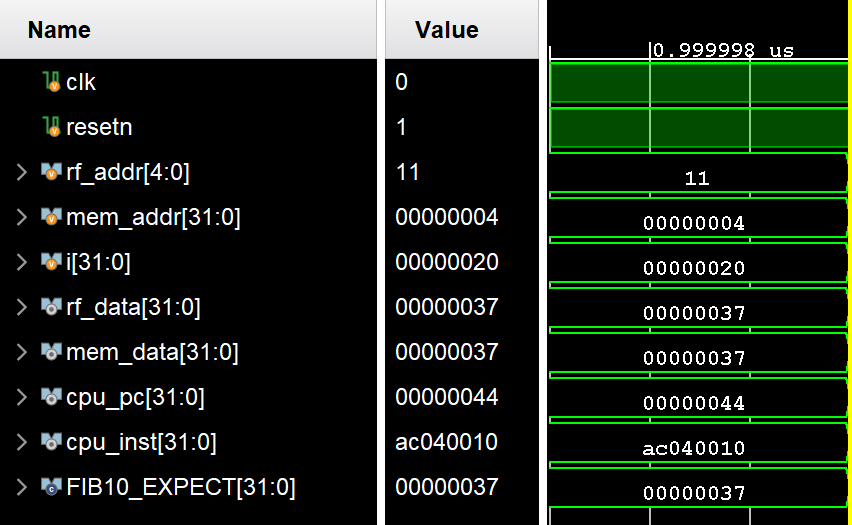
\includegraphics[width=\textwidth]{sim.png}
    \caption{仿真波形}
\end{figure}

\subsection{上板验证}
\begin{enumerate}
    \item 下载\texttt{single\_cycle\_cpu\_display.bit}；
    \item 运行Fibonacci程序，观察17号寄存器数据的变化
    \item 将内存观察地址设置为\texttt{1}（对应字节地址\texttt{4}）；
    \item 观察\texttt{mem\_data=0x00000037}，验证结果正确。
\end{enumerate}

\begin{figure}[!h]
    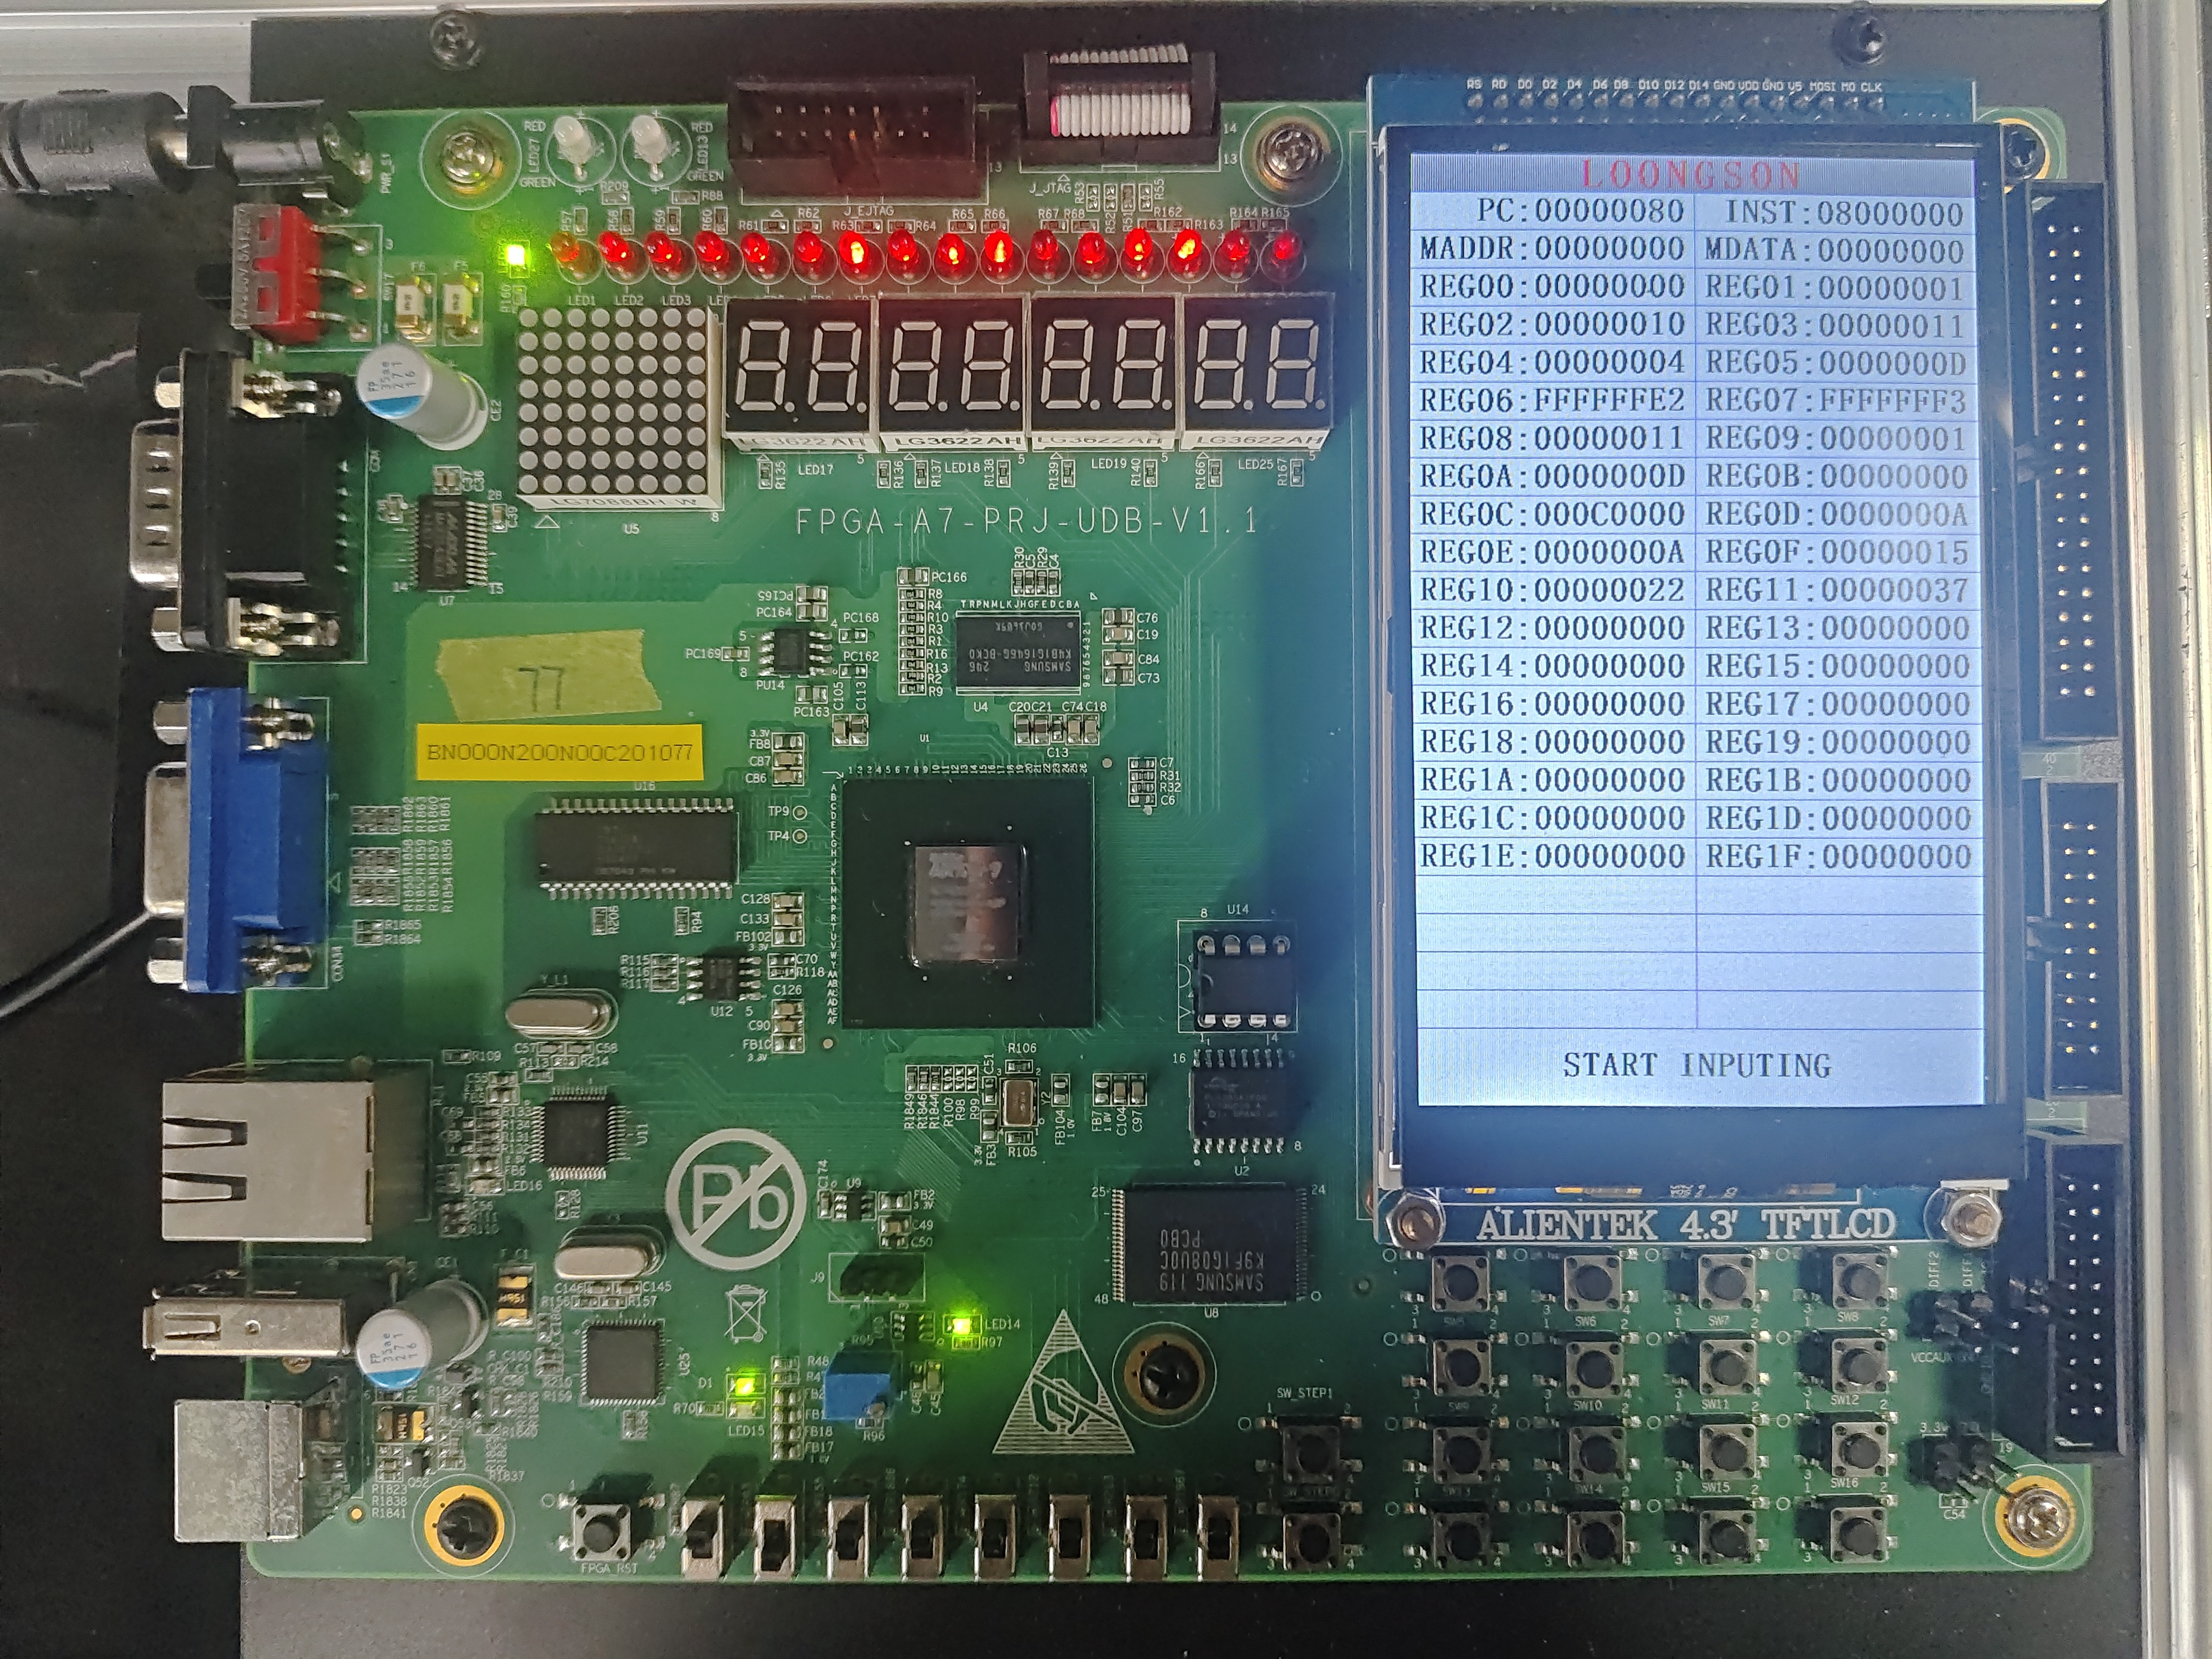
\includegraphics[width=\textwidth]{reg.jpg}
    \caption{上箱验证：观察17号寄存器}
\end{figure}

\begin{figure}[!h]
    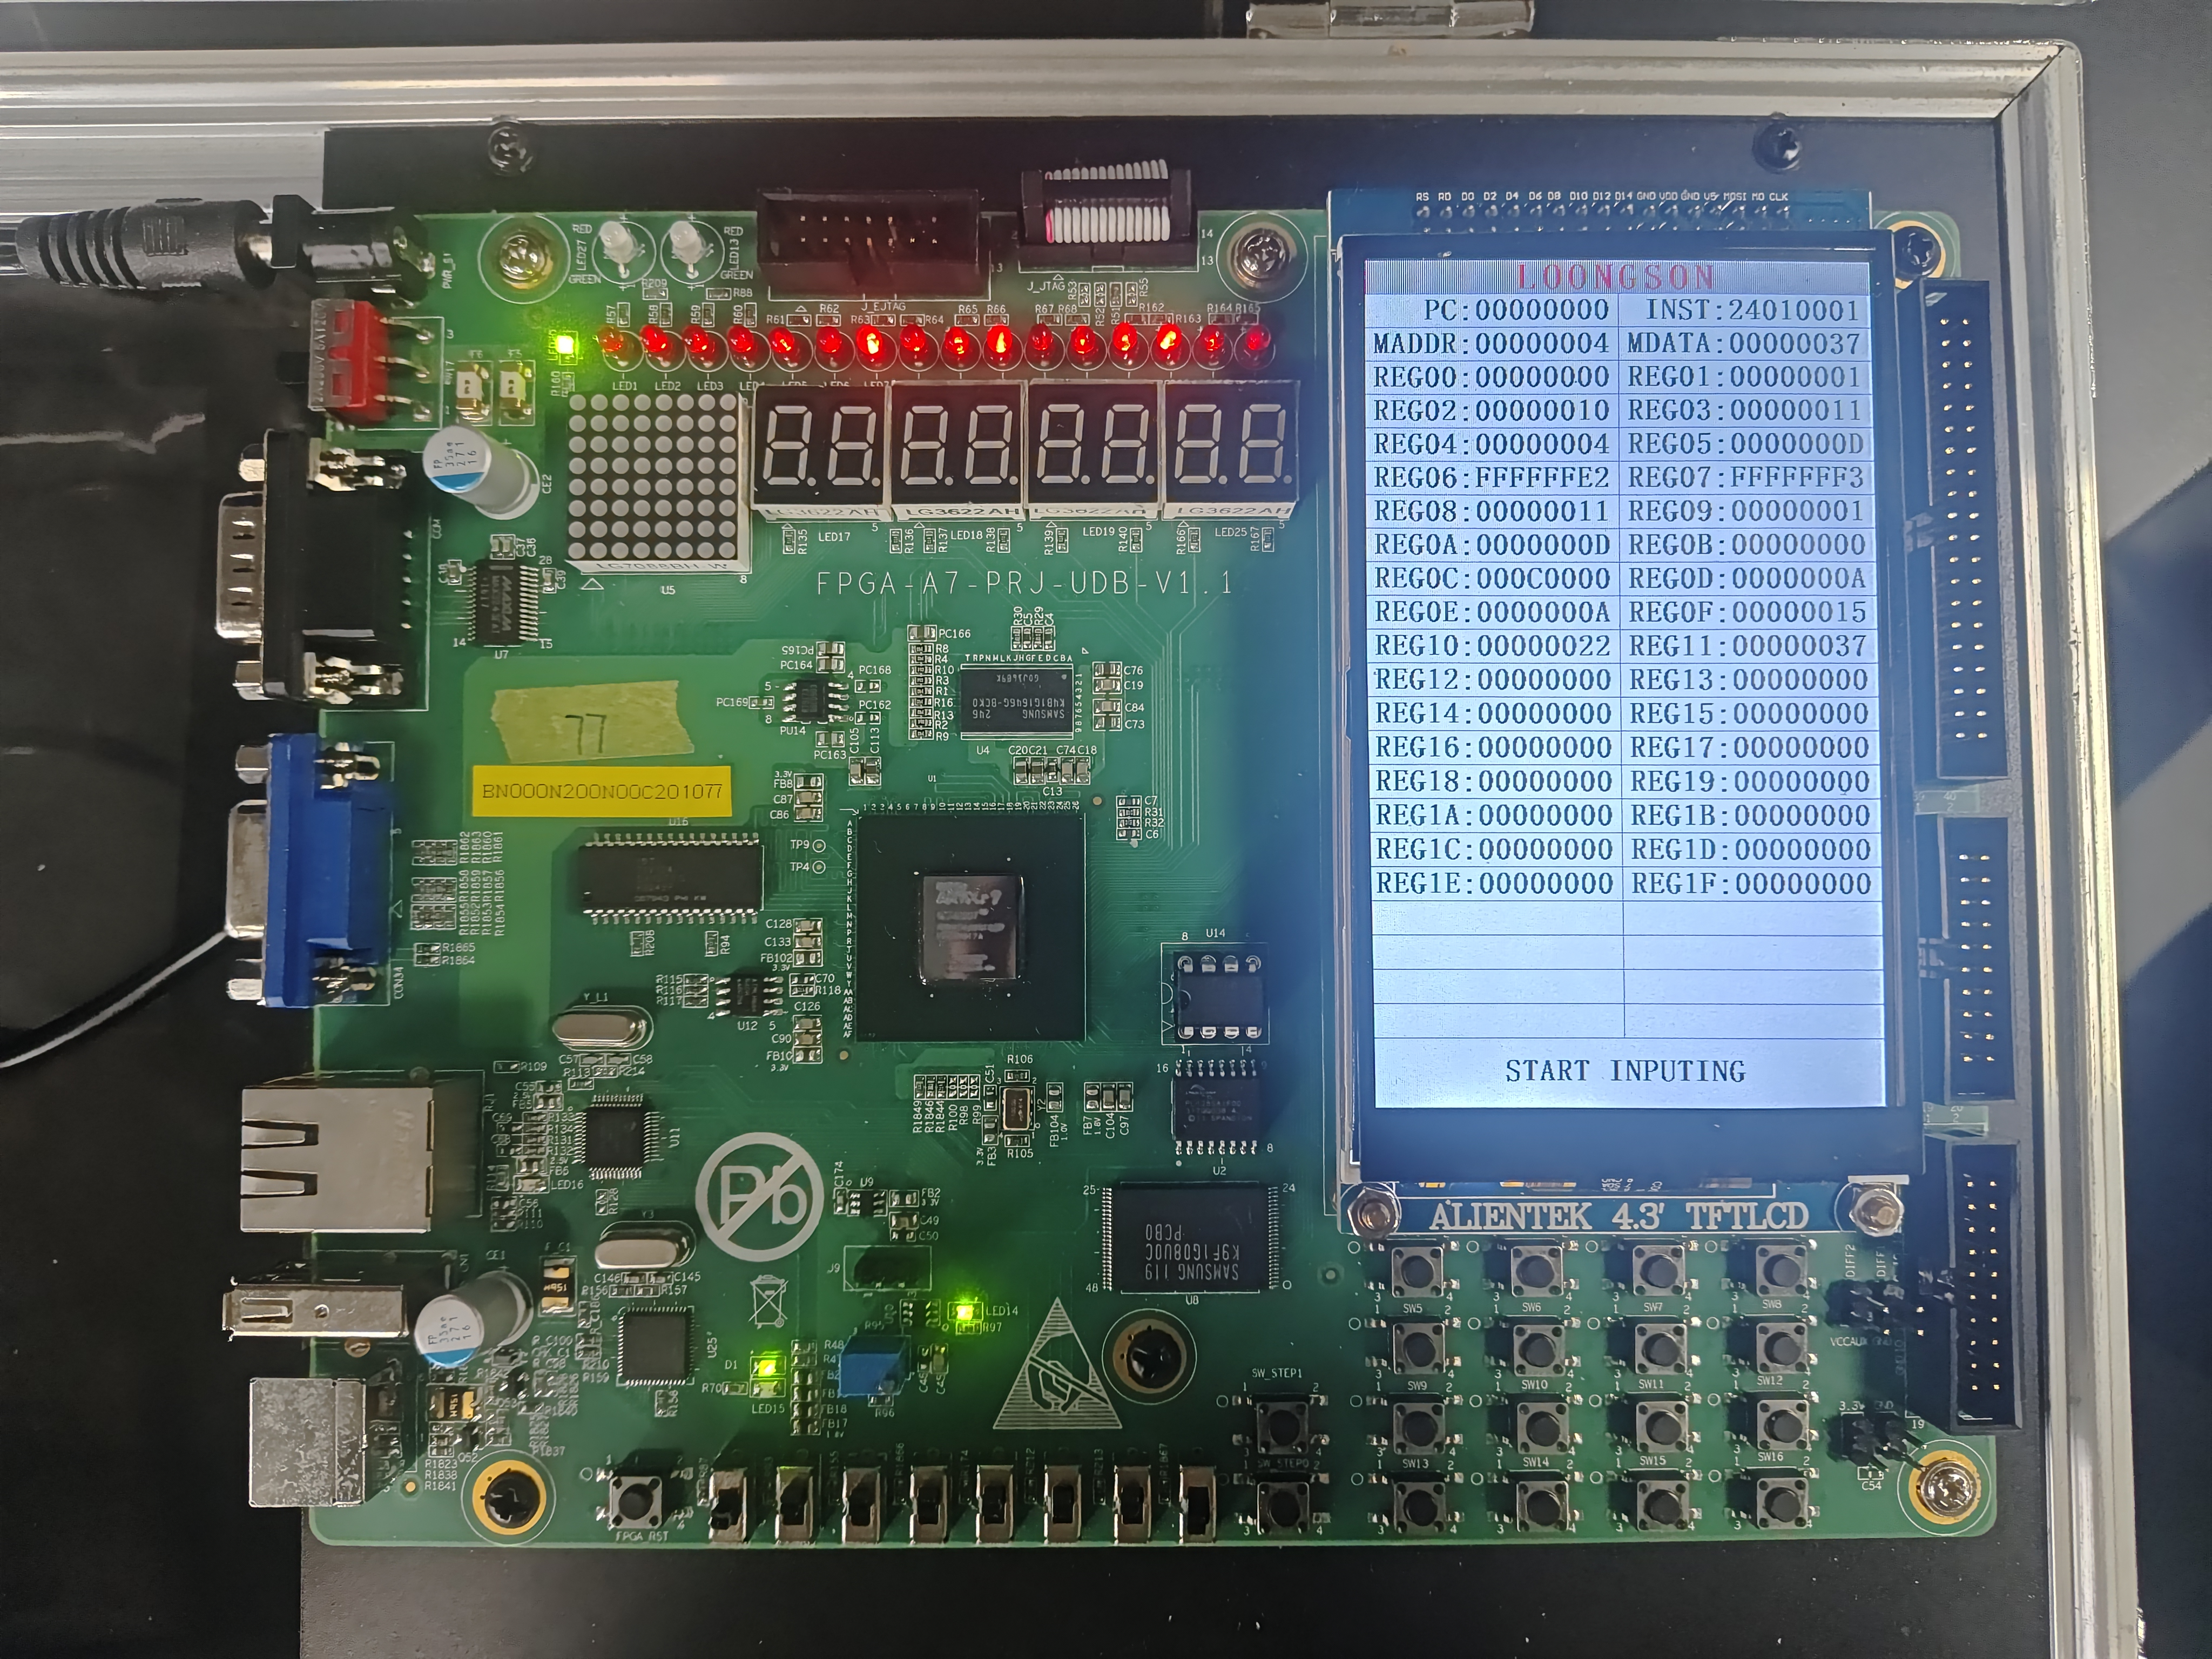
\includegraphics[width=\textwidth]{ram.jpg}
    \caption{上箱验证：从内存中读取结果}
\end{figure}

\newpage
\section{实验收获}
\begin{itemize}
   \item 理解了新增指令对译码、分支和写回路径的联动影响；
   \item 掌握了\texttt{bgtz}分支判定在硬件中的实现方法；
\end{itemize}

\section{附：源码目录}
\begin{itemize}
\item \verb|lab6/lab6.srcs/sources_1/imports/lab6/single_cycle_cpu.v|
\item \verb|lab6/lab6.srcs/sources_1/imports/lab6/inst_rom.v|
\item \verb|lab6/lab6.srcs/sources_1/imports/lab6/alu.v|
\item \verb|lab6/lab6.srcs/sim_1/imports/lab6/tb.v|
\item \verb|lab6/fibonacci3.asm|
\end{itemize}

\end{document}
